\chapter{Capa de Aplicación}
\label{chap:Aplicacion}
\textit{This chapter introduces the theoretical, experimental and computational concepts used throughout the thesis}
\vspace{2ex}\vfill
\minitoc
\newpage

\section{Punto de Vista Comportamiento de Aplicación}
El punto de vista del comportamiento de aplicaciones describe el comportamiento interno de la aplicación, este punto de vista es útil en el diseño del comportamiento principal de aplicaciones, o en la identificación de solapamiento funcional entre diferentes aplicaciones.

  \begin{table}[!h]
  	\centering
  	\begin{tabular}{lp{8cm}}
  		\toprule
  		\textbf{Nombre} & \textbf{Comportamiento de Aplicación} \\
  		\midrule
  		\textbf{Stakeholders} & Arquitectos de la organización, proceso, aplicación y dominio \\
  		\textbf{Preocupaciones} & Estructurar las relaciones entre las aplicaciones, garantizar la consistencia e integridad, reducir la complejidad \\
  		\textbf{Propósito} & Diseñar \\
  		\textbf{Nivel de Abstracción} & Coherencia, detalle \\
  		\textbf{Capa} & Capa de Aplicación (Aplicación) \\
  		\textbf{Aspectos} & Activo, comportamiento, (información) \\
  		\bottomrule
  	\end{tabular}
	\captionsetup{width=.95\textwidth}
	\caption{Descripción punto de vista comportamiento de aplicación}
	\label{tabla10}
  \end{table}

  \begin{figure}[!h]
	\centering
	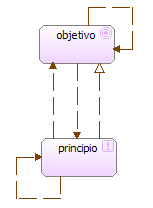
\includegraphics[scale=0.2]{figuras/20.png}
	\captionsetup{width=.95\textwidth}
	\caption{Posición del punto de vista comportamiento de aplicación conceptualmente y marco del punto de vista}
	\label{figura20}
  \end{figure}

\subsection{Metamodelo}
En la Figura 7.1 se ilustra el metamodelo perteneciente al punto de vista comportamiento de aplicación, el concepto clave para la estructura es el componente de aplicación, a este componentes se le asignan funciones de aplicación, las cuales realizan los servicios de aplicación donde estos servicios soportan los procesos de negocio, se generan unos objetos de datos; la interface es la encargada de interconectar los componentes, en el metamodelo aparece la colaboración de aplicación donde se reúnen componentes que aplican el concepto
de colaboración.

\begin{figure}[!h]
	\centering
	\includegraphics{metamodelos/7.png}
	\captionsetup{width=.95\textwidth}
	\caption{Metamodelo punto de vista comportamiento de aplicación}
	\label{metamodelo7}
\end{figure}

\subsection{Modelo mInstituto}Chachara del diagrama
\begin{figure}[!h]
	\centering
	\includegraphics{modelos/7.png}
	\captionsetup{width=.95\textwidth}
	\caption{Modelo punto de vista comportamiento de aplicación: minstituto}
	\label{modelo7}
\end{figure}

\section{Punto de Vista Cooperación de Aplicación}
El punto de vista de Cooperación de la aplicación describe las relaciones entre los componentes de las aplicaciones en función de los flujos de información entre ellos, o en términos de los servicios que ofrecen y su uso. Este punto de vista también se utiliza para expresar la cooperación (interna) o la orquestación de los servicios que en conjunto apoyan la ejecución de un proceso de negocio.

  \begin{table}[!h]
  	\centering
  	\begin{tabular}{lp{8cm}}
  		\toprule
  		\textbf{Nombre} & \textbf{Cooperación de Aplicación} \\
  		\midrule
  		\textbf{Stakeholders} & Arquitectos de la organización, proceso, aplicación y dominio \\
  		\textbf{Preocupaciones} & Estructurar las relaciones y dependencias entre las aplicaciones, orquestación de los servicios, garantizar la consistencia e integridad, reducir la complejidad \\
  		\textbf{Propósito} & Diseñar \\
  		\textbf{Nivel de Abstracción} & Coherencia, detalle \\
  		\textbf{Capa} & Capa de Aplicación (Aplicación) \\
  		\textbf{Aspectos} & Activo, comportamiento \\
  		\bottomrule
  	\end{tabular}
  	\captionsetup{width=.95\textwidth}
  	\caption{Descripción punto de vista cooperación de aplicación}
  	\label{tabla11}
  \end{table}

\begin{figure}[!h]
	\centering
	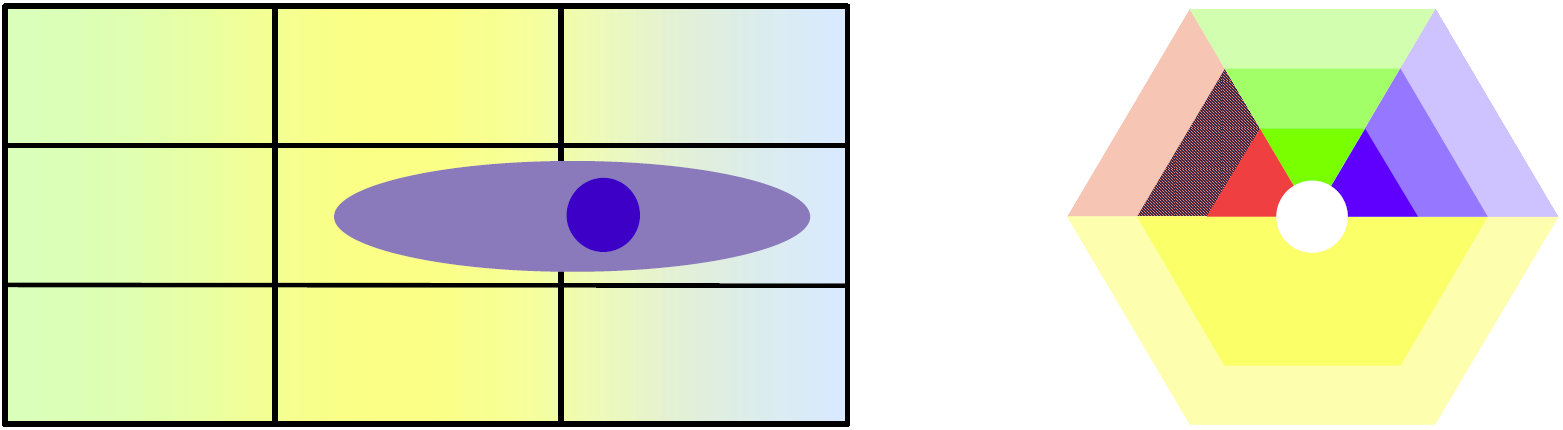
\includegraphics[scale=0.2]{figuras/21.png}
	\captionsetup{width=.95\textwidth}
	\caption{Posición del punto de vista cooperación de aplicación conceptualmente y marco del punto de vista}
	\label{figura21}
\end{figure}

\subsection{Metamodelo}
En la figura Figura 7.3 se ilustra el metamodelo perteneciente al punto de vista cooperación de aplicación, el punto de vista se centra en la localización,ya que se agrupan los componentes en un front office y un back office.

\begin{figure}[!h]
	\centering
	\includegraphics{metamodelos/8.png}
	\captionsetup{width=.95\textwidth}
	\caption{Metamodelo punto de vista cooperación de aplicación}
	\label{metamodelo8}
\end{figure}

\subsection{Modelo mInstituto}Chachara del diagrama
\begin{figure}[!h]
	\centering
	\includegraphics{modelos/8.png}
	\captionsetup{width=.95\textwidth}
	\caption{Modelo Punto de Vista Cooperación de Aplicación: minstituto}
	\label{modelo8}
\end{figure}

\section{Punto de Vista Estructura de Aplicación}
El punto de vista de estructura de la aplicación, muestra la estructura de componentes de una aplicación Este punto de vista es útil en el diseño o la comprensión de la estructura principal de componentes de la aplicación y el uso de datos asociados.

  \begin{table}[!h]
  	\centering
  	\begin{tabular}{lp{8cm}}
  		\toprule
  		\textbf{Nombre} & \textbf{Estructura de Aplicación} \\
  		\midrule
  		\textbf{Stakeholders} & Arquitectos de la organización, aplicación y dominio \\
  		\textbf{Preocupaciones} & Estructura de la aplicación, garantizar la consistencia e integridad, reducir la complejidad \\
  		\textbf{Propósito} & Diseñar \\
  		\textbf{Nivel de Abstracción} & Detalle \\
  		\textbf{Capa} & Capa de Aplicación \\
  		\textbf{Aspectos} & Activo, (Pasivo) \\
  		\bottomrule
  	\end{tabular}
  	\captionsetup{width=.95\textwidth}
  	\caption{Descripción punto de vista estructura de aplicación}
  	\label{tabla12}
  \end{table}

  \begin{figure}[!h]
	\centering
	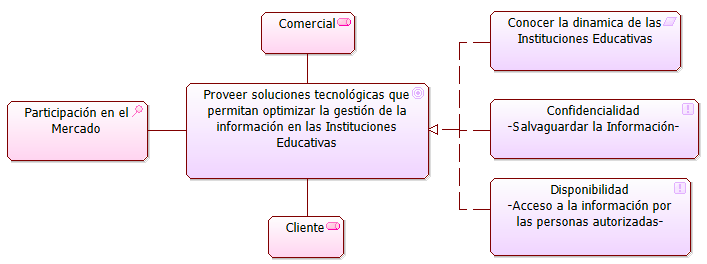
\includegraphics[scale=0.2]{figuras/22.png}
	\captionsetup{width=.95\textwidth}
	\caption{Posición del punto de vista estructura de aplicación conceptualmente y marco del punto de vista}
	\label{figura22}
  \end{figure}

  \subsection{Metamodelo}
  En la figura Figura 7.5 se ilustra el metamodelo perteneciente al punto de vista de estructura de la aplicación en este metamodelo se involucran el componente y la interfaz, se muestra la forma de interactuar el sistema con los componentes de software haciendo uso de las interfaces de comunicación.

  \begin{figure}[!h]
	\centering
	\includegraphics{metamodelos/9.png}
	\captionsetup{width=.95\textwidth}
	\caption{Metamodelo punto de vista estructura de aplicación}
	\label{metamodelo9}
  \end{figure}

  \subsection{Modelo mInstituto}Chachara del diagrama
  \begin{figure}[!h]
	\centering
	\includegraphics{modelos/9.png}
	\captionsetup{width=.95\textwidth}
	\caption{Modelo punto de vista estructura de aplicación: minstituto}
	\label{modelo9}
  \end{figure}
  
  \section{Punto de Vista de Uso de Aplicación}
  El punto de vista de uso de aplicación describe como las aplicaciones son usadas para soportar uno o mas procesos de negocio, y como ellos son usados por otras aplicaciones. Puede ser usado en el diseño de una aplicación para identificar los servicios requeridos por los procesos de negocios y otras aplicaciones, o en el diseño de procesos de negocio para describir los servicios que están disponibles. Así, al identificar las dependencias de los procesos de negocio sobre las aplicaciones, puede ser útil para los administradores operativos responsables de estos procesos.
  
  \begin{table}[!h]
  	\centering
  	\begin{tabular}{lp{8cm}}
  		\toprule
  		\textbf{Nombre} & \textbf{Uso de aplicación} \\
  		\midrule
  		\textbf{Stakeholders} & La empresa, el proceso, los arquitectos de aplicaciones, directores de operaciones \\
  		\textbf{Preocupaciones} & Consistencia e Integridad, Reducción de la complejidad \\
  		\textbf{Propósito} & Diseñar, decidir \\
  		\textbf{Nivel de Abstracción} & Coherencia \\
  		\textbf{Capa} & Capa de Negocio y Aplicación \\
  		\textbf{Aspectos} & Comportamiento, estructura \\
  		\bottomrule
  	\end{tabular}
  	\captionsetup{width=.95\textwidth}
  	\caption{Descripción punto de vista de Uso de Aplicación}
  	\label{tabla13}
  \end{table}
  
  \begin{figure}[!h]
  	\centering
  	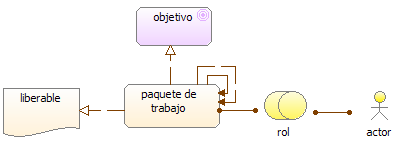
\includegraphics[scale=0.2]{figuras/23.png}
  	\captionsetup{width=.95\textwidth}
  	\caption{Posición del punto de vista de Uso de Aplicación conceptualmente y marco del punto de vista}
  	\label{figura23}
  \end{figure}
  
  \subsection{Metamodelo}
  En la figura Figura 7.5 se ilustra el metamodelo perteneciente al punto de vista de Uso de Aplicación en este metamodelo se involucran el componente y la interfaz, se muestra la forma de usar el software haciendo uso de las interfaces y componentes.
  
  \begin{figure}[!h]
  	\centering
  	\includegraphics{metamodelos/10.png}
  	\captionsetup{width=.95\textwidth}
  	\caption{Metamodelo punto de vista de Uso de Aplicación}
  	\label{metamodelo10}
  \end{figure}
  
  \subsection{Modelo mInstituto}Chachara del diagrama
  \begin{figure}[!h]
  	\centering
  	\includegraphics{modelos/10.png}
  	\captionsetup{width=.95\textwidth}
  	\caption{Modelo punto de vista de Uso de Aplicación: minstituto}
  	\label{modelo10}
  \end{figure}